\subsection{Jet Cleaning}
\label{sec:GBJ2:Cleaning}

The analysis removes events with jets that have $\pt{}>20$ GeV  and that fail the loose cleaning cut.
This event-level jet cleaning cut can be compared to a jet-level cleaning cut, which only removes the jets that fail the loose cleaning cuts, to assess the impact of rejecting events due to bad jets.



Figure \ref{GBJ2:JetCleaning:gap} shows the ratio of jet-level to event-level cleaning criteria for the loose cleaning cuts on (a) the gap fraction and (b) the average number of jets in the rapidity region bounded by the dijet as a function of \dy{}.
The effect on the gap fraction is negligible throughout \dy{}, with fluctuations of less than half a percent across the \dy{} range but with no net bias.
The effect on the average number of jets is small throughout \dy{} with fluctuations below half a percent.

Figure \ref{GBJ2:JetCleaning:cos} and \ref{GBJ2:JetCleaning:cos2} shows the ratio of jet-level to event-level cleaning criteria for the loose cleaning cuts  on the \mean{\cosdphi{}} and the \mean{\costwodphi{}} respectively as a function of \dy{} for both (a) inclusive events and (b) gap events.
The effect on the \mean{\cosdphi{}} and \mean{\costwodphi{}} is negligible for both inclusive and gap events.

Figure \ref{GBJ2:JetCleaning:dphi23} shows the ratio of jet-level to event-level cleaning criteria for the loose cleaning cuts on \dphiDist{} for (a) inclusive events and (b) gap events for $2<\dy{}<3$. 
The effect is of the order of half a percent which is negligible, especially compared to statistical and other systematic uncertainties.
There are similar results for the other \dy{} slices.

The cross-section distributions show the largest effect, as the event-level cleaning cut will remove more event. 
This difference is less than half a percent, and the systematic uncertainty due to this is negligible.
The other distributions show negligible differences when changing from an event-level cleaning criteria to a jet-level cleaning criteria. 
Event-level cleaning was determined to have no bias and is used in the final analysis. 





Loose jet cleaning does not remove all of the bad jets, and to assess the effect from the remaining bad jets, the final distributions are compared to the more stringent ``medium'' jet cleaning, which  removes a higher proportion of bad jets. 
The concern with using the medium jet cleaning cut is that it has inefficiencies for good jets that have a low \pt{}.
These inefficiencies have been estimated in \cite{ref:JES}.
The differences from comparing the medium and loose cleaning cuts will come from removing more bad jets and the good jet inefficiencies.
To try to isolate the effect due to the bad jets on each distribution, the medium jet cleaning cuts are compared to events that have the inefficiencies from \cite{ref:JES} applied to events selected using the loose cleaning cuts, termed ``inefficient loose cleaning''. 


Figure \ref{GBJ2:JetCleaning:gap_ML} shows the ratio of the gap fraction as a function of (a) \dy{} and (b) \qz{} for  $2<\dy{}<3$,  for the medium cleaning to the loose cleaning.
Also shown is the ratio of inefficient loose cleaning to the loose cleaning.
Changing to the medium cleaning causes the gap fraction to increase with a maximum difference of $\approx 2\%$ at high \dy{} and $\approx 1\%$ at low \qz{}.
This increase in the gap fraction results from gap events having less jets than inclusive events, meaning they are less likely to fail the jet cleaning cut. 
The inefficient loose cleaning matches the medium data well, which would indicate that the effect from bad jets on the gap fraction is small and the main effect is from the good jet inefficiency. 
Similar results are seen for the gap fraction against \qz{} in the other slices in \dy{}.  


The ratio of the medium cleaning to the loose cleaning and the inefficient loose cleaning to the loose cleaning for event-level criteria is shown in Figures \ref{GBJ2:JetCleaning:cos_ML} and \ref{GBJ2:JetCleaning:cos2_ML} for \mean{\cosdphi{}} and \mean{\costwodphi{}} respectively as a function of \dy{} for (a) inclusive events and (b) events that pass the jet veto. 
Both distributions show that the effect of the bad jets and inefficiency is small for both gap and inclusive events.
At larger \dy{} there are some statistical fluctuation.

Figure \ref{GBJ2:JetCleaning:dphi23_ML} shows the ratio of \dphiDist for $2<\dy{}<3$ for the medium cleaning to the loose cleaning, and the ratio of inefficient loose cleaning to the loose cleaning for (a) inclusive events and (b) events that pass the jet veto.
There is a reduction of $\approx 2\%$ in the gap and inclusive cross-section when the medium cleaning cut is applied.
The inefficient loose cleaning cuts causes a reduction to \dphiDist{} of between $2-4\%$, and crucially it falls to below the medium jet cleaning ratio. 
This indicates that the inefficiencies of the medium jet cleaning on good jets are overestimated.
The maximum effect from the bad jets would occur if there was no inefficiency in the medium jet cleaning, ie corresponding to the deviation of the distribution from unity. 
For the slice of $2<\dy{}<3$, the maximum deviation is $3\%$, which would be a very conservative estimate of the effect.
Given that this is an overestimation of a effect that is expected to be small, and the uncertainty from the JES adds an uncertainty band of about $20\%$, this difference is disregarded. 
The other slices in \dy{} show a similar results when comparing the difference between medium jet cleaning and loose cleaning to the systematic band from JES.


The method of jet cleaning used this analysis was the loose cleaning definitions and event-level criteria.
No bias due to using event-level was found. 
The loose cleaning definition was used due to the high efficiency for good jets.
The effect from bad jets was assessed, and while it is hard to get an accurate value for the effect due to the medium jet inefficiencies for good jets being overestimated, the upper limit of the effect was significantly less than the effect from the JES uncertainty. 
No systematic uncertainty from cleaning is applied for the final analysis.


\begin{figure}
\centering
        \begin{subfigure}[b]{0.5\textwidth}
                \centering
                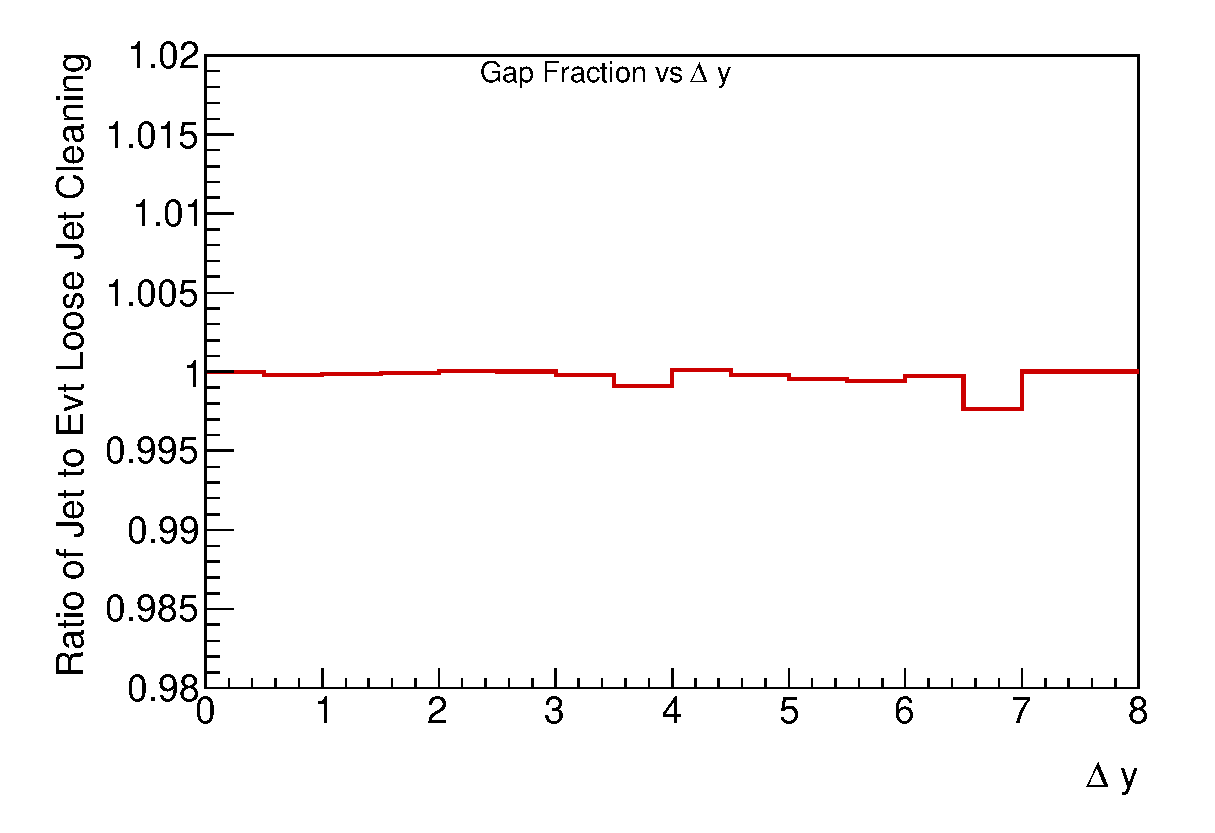
\includegraphics[width=\textwidth]{figures/GBJ2/jetcleaning/Clean___GapFraction_deltaY_Ratio_Loose_JetEvt_Data.eps}
        \end{subfigure}%
        \begin{subfigure}[b]{0.5\textwidth}
                \centering
                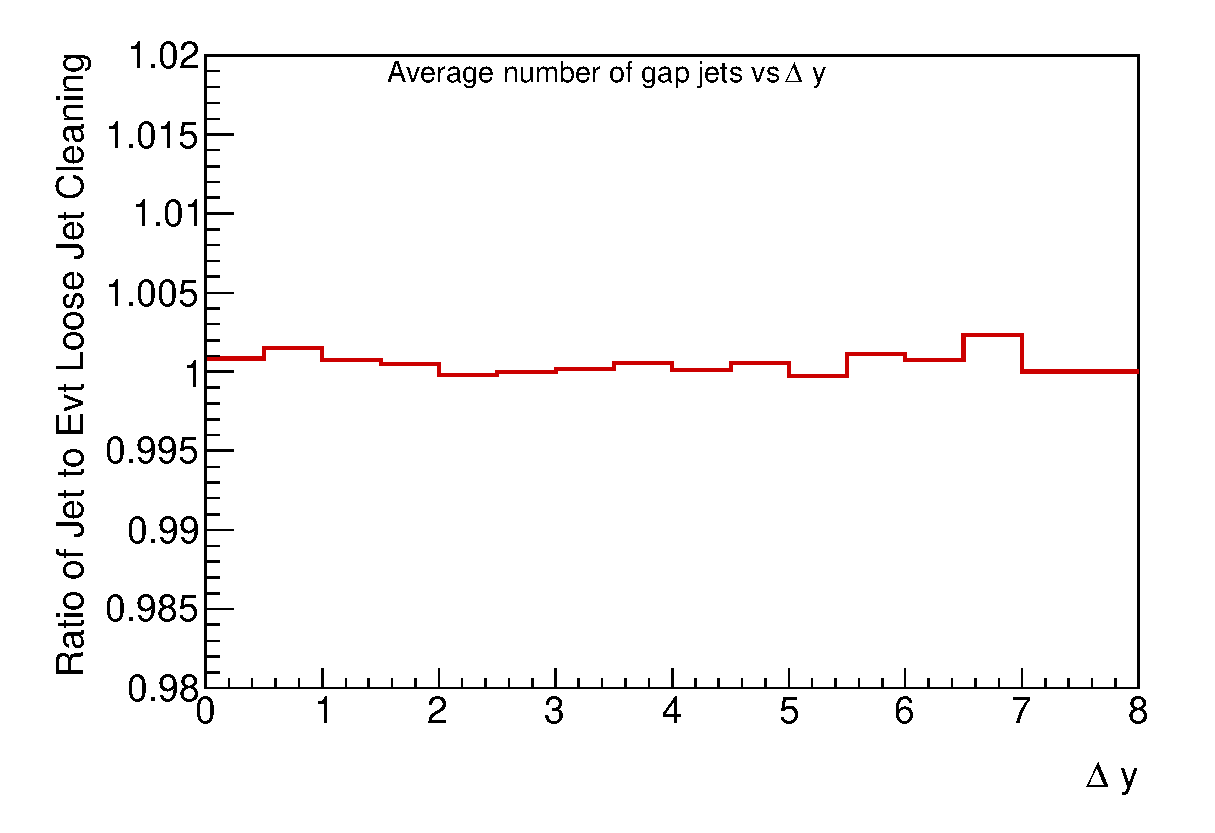
\includegraphics[width=\textwidth]{figures/GBJ2/jetcleaning/Clean___prof_deltaY_njets_Ratio_Loose_JetEvt_Data.eps}
        \end{subfigure}%
\caption[Comparison between event and jet level cleaning cuts on the gap fraction and average number of jets]{
The ratio of (a) the gap fraction and (b) average number of jets in the gap region as a function of \dy{} for the data with jet-level cleaning cuts compared to the data with event-level cleaning cuts.
\label{GBJ2:JetCleaning:gap}}
\end{figure}


\begin{figure}
\centering
        \begin{subfigure}[b]{0.5\textwidth}
                \centering
                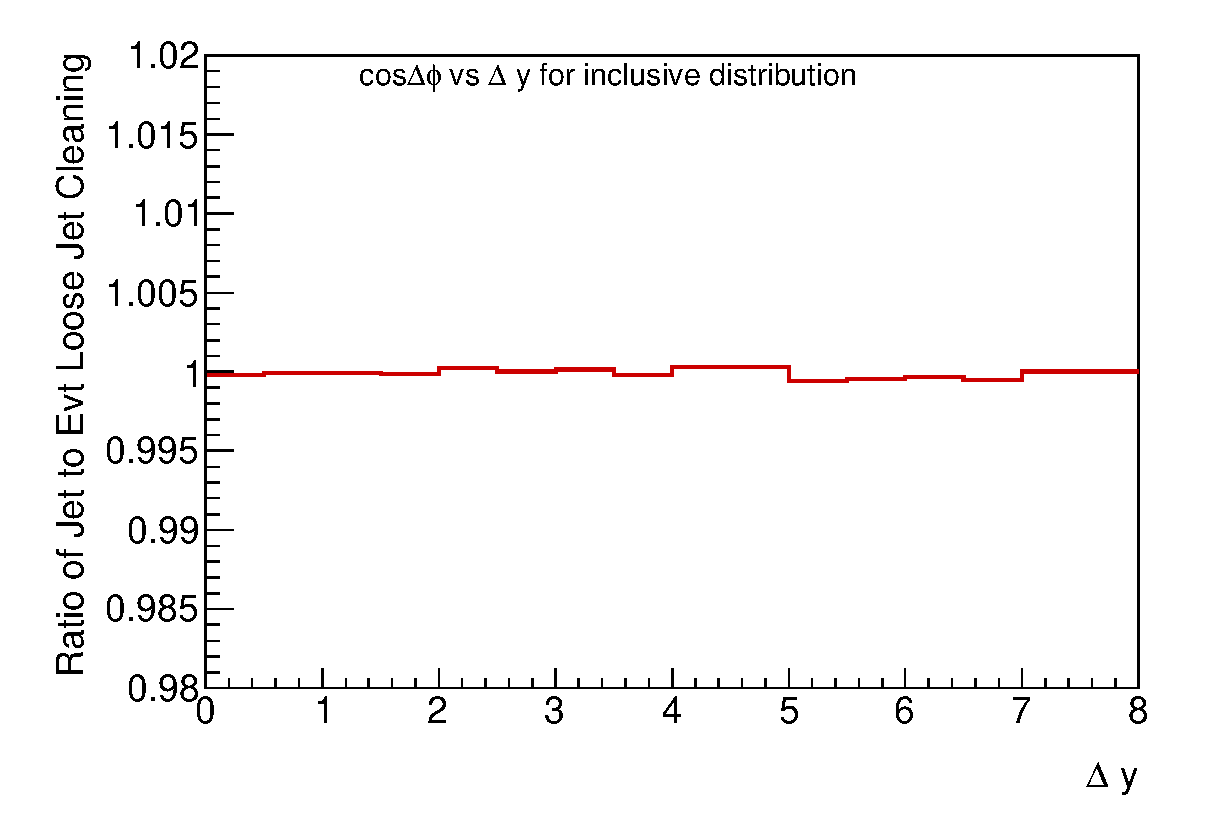
\includegraphics[width=\textwidth]{figures/GBJ2/jetcleaning/Clean___cosdPhi_deltaY_Ratio_Loose_JetEvt_Data.eps}
        \end{subfigure}%
        \begin{subfigure}[b]{0.5\textwidth}
                \centering
                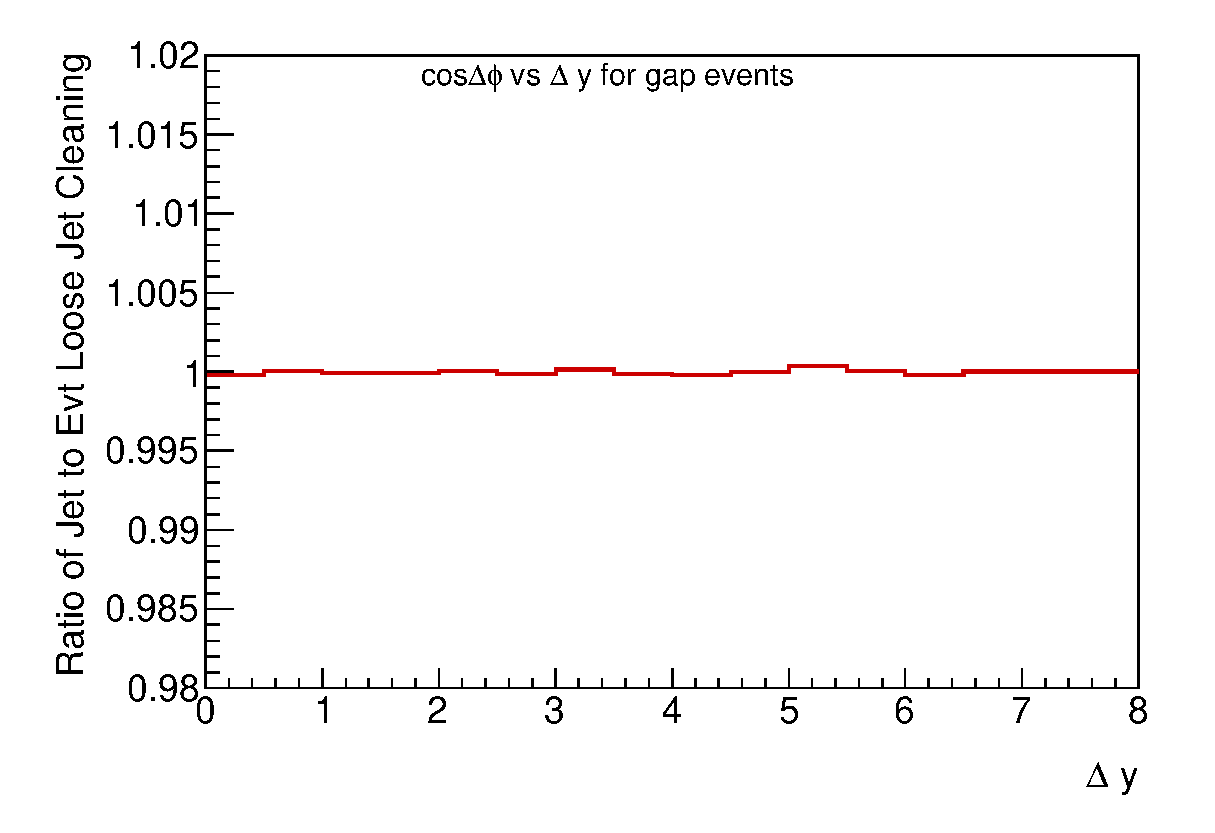
\includegraphics[width=\textwidth]{figures/GBJ2/jetcleaning/Clean___cosdPhi_deltaY_gap_Ratio_Loose_JetEvt_Data.eps}
        \end{subfigure}%
\caption[Comparison between event and jet level cleaning cuts on the \mean{\cosdphi{}}]{
The ratio of \mean{\cosdphi{}} as a function of \dy{} for (a) inclusive and (b) gap events for the data with jet-level cleaning cuts compared to the data with event-level cleaning cuts.
\label{GBJ2:JetCleaning:cos}}
\end{figure}


\begin{figure}
\centering
        \begin{subfigure}[b]{0.5\textwidth}
                \centering
                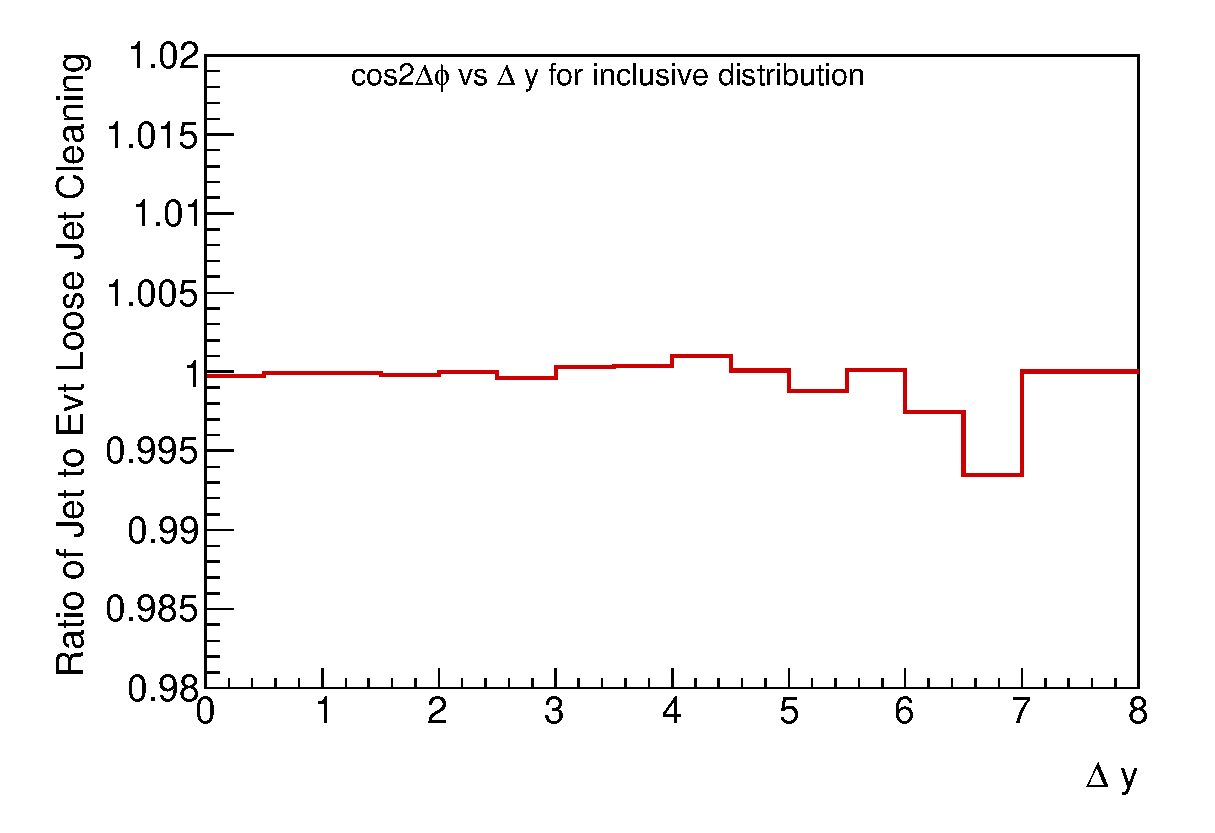
\includegraphics[width=\textwidth]{figures/GBJ2/jetcleaning/Clean___cos2dPhi_deltaY_Ratio_Loose_JetEvt_Data.eps}
        \end{subfigure}%
        \begin{subfigure}[b]{0.5\textwidth}
                \centering
                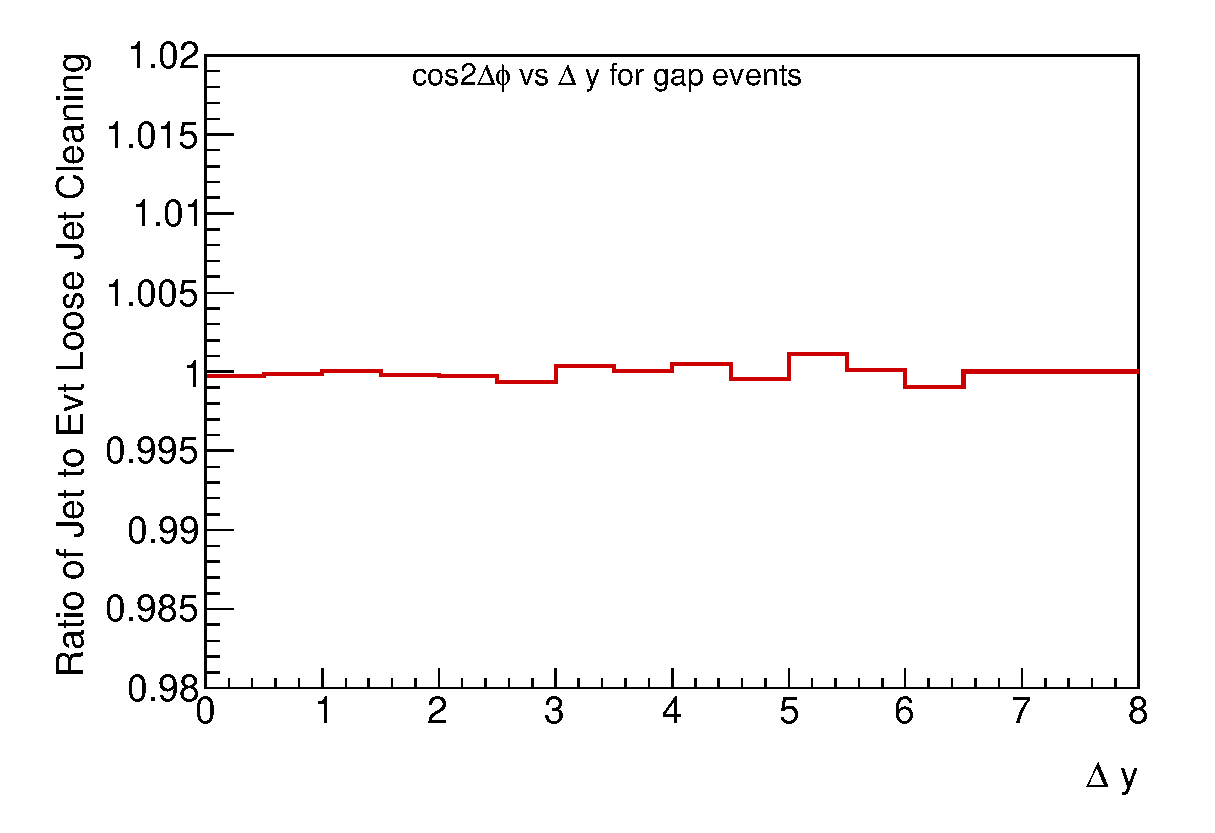
\includegraphics[width=\textwidth]{figures/GBJ2/jetcleaning/Clean___cos2dPhi_deltaY_gap_Ratio_Loose_JetEvt_Data.eps}
        \end{subfigure}%
\caption[Comparison between event and jet level cleaning cuts on the \mean{\costwodphi{}}]{
The ratio of \mean{\costwodphi{}} as a function of \dy{} for (a) inclusive and (b) gap events for the data with jet-level cleaning cuts compared to the data with event-level cleaning cuts.

\label{GBJ2:JetCleaning:cos2}}
\end{figure}


\begin{figure}
\centering
        \begin{subfigure}[b]{0.5\textwidth}
                \centering
                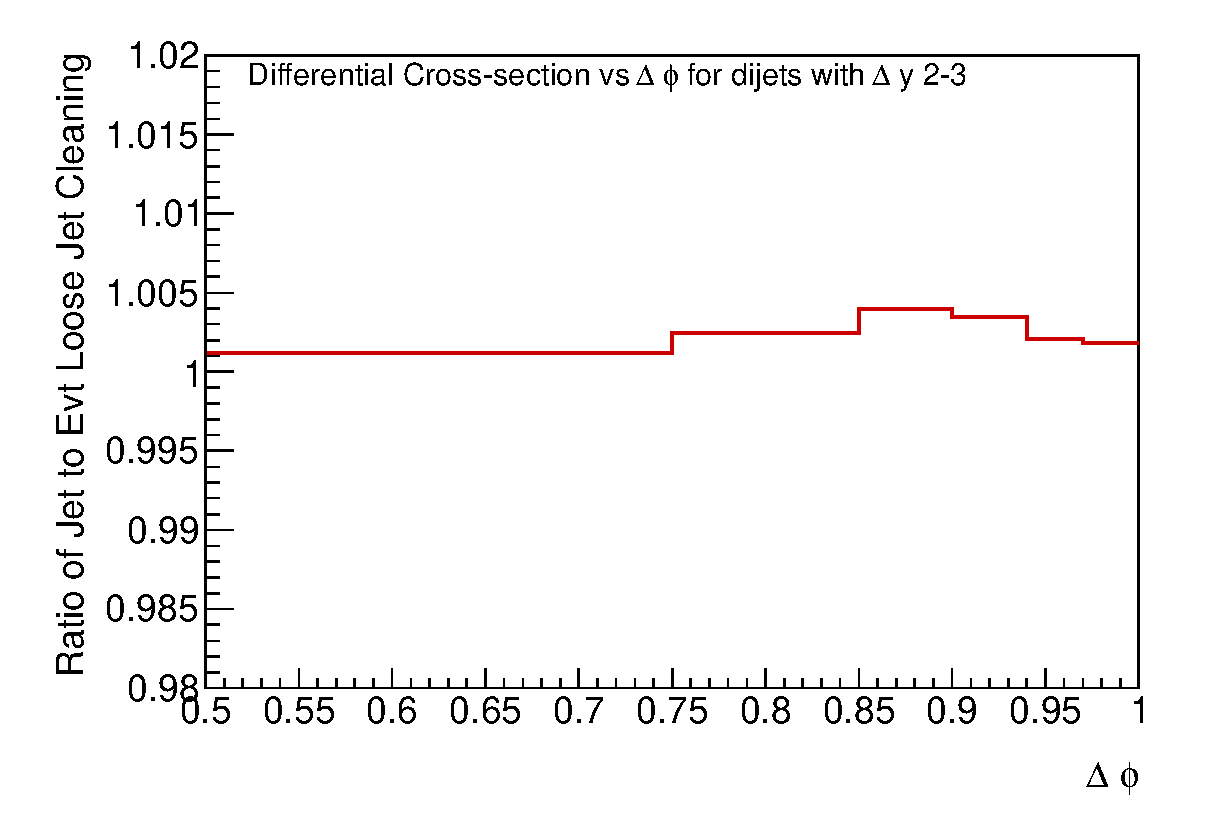
\includegraphics[width=\textwidth]{figures/GBJ2/jetcleaning/Clean___dPhi__2_3_Ratio_Loose_JetEvt_Data.eps}
        \end{subfigure}%
        \begin{subfigure}[b]{0.5\textwidth}
                \centering
                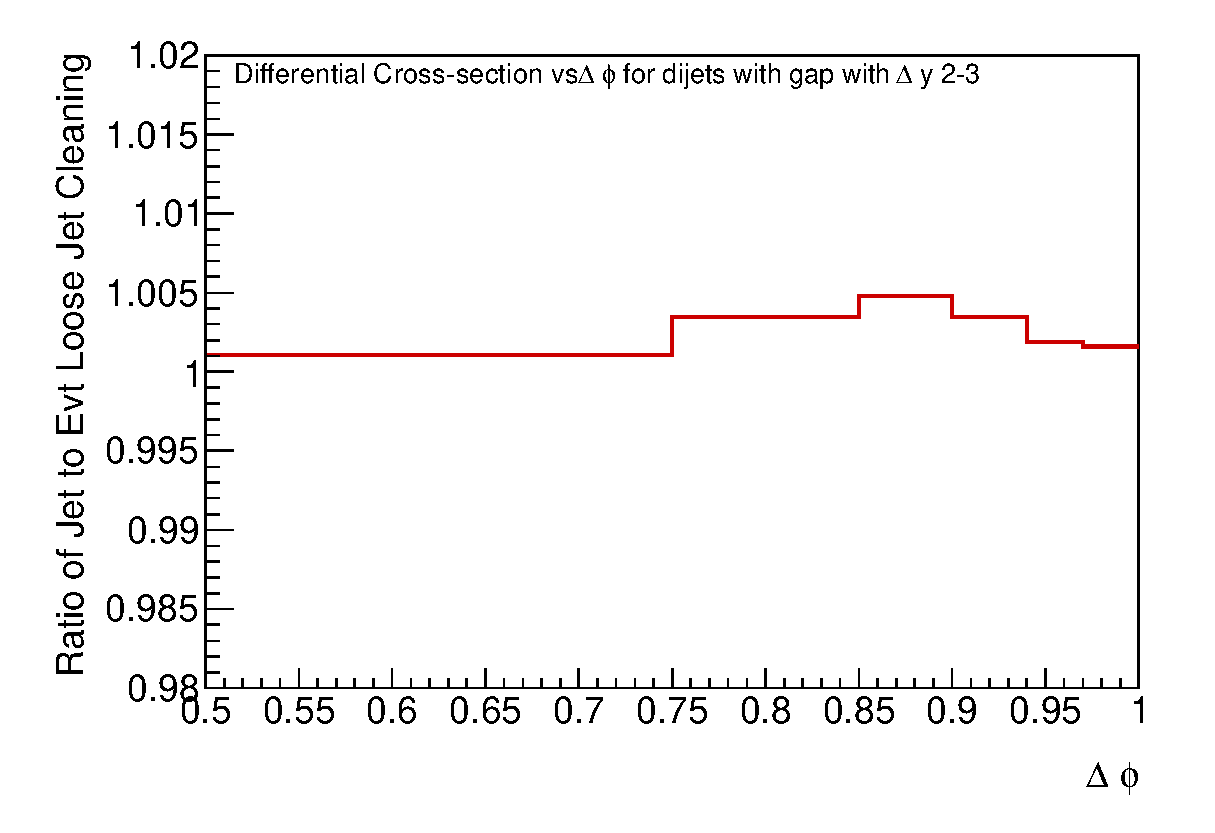
\includegraphics[width=\textwidth]{figures/GBJ2/jetcleaning/Clean___dPhi_gap__2_3_Ratio_Loose_JetEvt_Data.eps}
        \end{subfigure}%
\caption[Comparison between event and jet level cleaning cuts on the \dphiDist{}]{

The ratio of \dphiDist{} for $2<\dy{}<3$ for (a) inclusive and (b) gap events for the data with jet-level cleaning cuts compared to the data with event-level cleaning cuts.

\label{GBJ2:JetCleaning:dphi23}}
\end{figure}



%\begin{figure}
%\centering
%\mbox{
%              \subfigure[]{\epsfig{figure=figures/GBJ2/jetcleaning/Clean___dPhi__4_5_Ratio_Loose_JetEvt_Data.eps,width=0.5\textwidth}}\quad
%              \subfigure[]{\epsfig{figure=figures/GBJ2/jetcleaning/Clean___dPhi_gap__4_5_Ratio_Loose_JetEvt_Data.eps,width=0.5\textwidth}}\quad
%                              }
%\caption[]{
%The ratio of the \dphi{} distribution for \dy{} of 4--5 for (a) inclusive and (b) gap events for the data with jet-level cleaning cuts compared to the data with event-level cleaning cuts.
%
%\label{GBJ2:JetCleaning:dphi45}}
%\end{figure}
%
%
%
%\begin{figure}
%\centering
%\mbox{
%              \subfigure[]{\epsfig{figure=figures/GBJ2/jetcleaning/Clean___dPhi__7_8_Ratio_Loose_JetEvt_Data.eps,width=0.5\textwidth}}\quad
%              \subfigure[]{\epsfig{figure=figures/GBJ2/jetcleaning/Clean___dPhi_gap__7_8_Ratio_Loose_JetEvt_Data.eps,width=0.5\textwidth}}\quad
%                              }
%\caption[]{
%The ratio of the \dphi{} distribution for \dy{} of 4--5 for (a) inclusive and (b) gap events for the data with jet-level cleaning cuts compared to the data with event-level cleaning cuts.
%
%\label{GBJ2:JetCleaning:dphi78}}
%\end{figure}
%

\begin{figure}
\centering
        \begin{subfigure}[b]{0.5\textwidth}
                \centering
                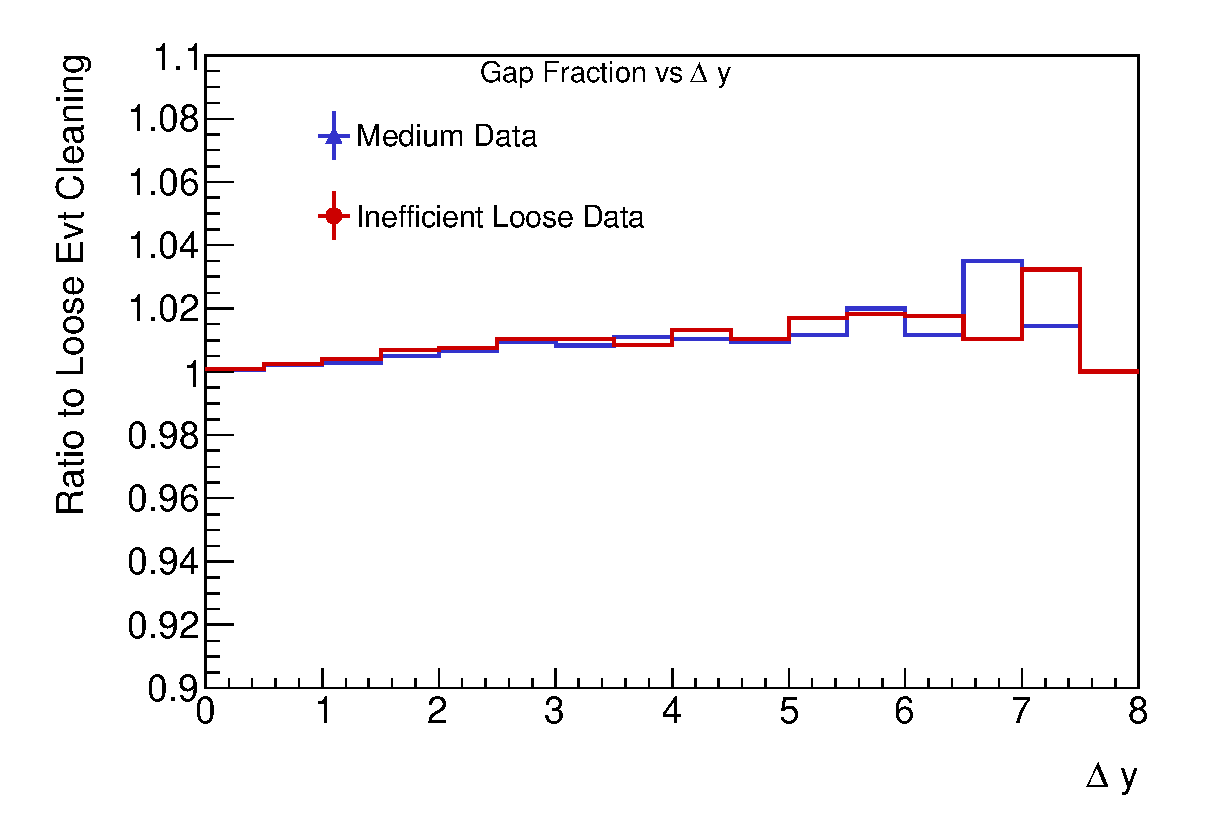
\includegraphics[width=\textwidth]{figures/GBJ2/jetcleaning/Clean___GapFraction_deltaY_Ratio_MediumLoose_Evt_Data.eps}
        \end{subfigure}%
        \begin{subfigure}[b]{0.5\textwidth}
                \centering
                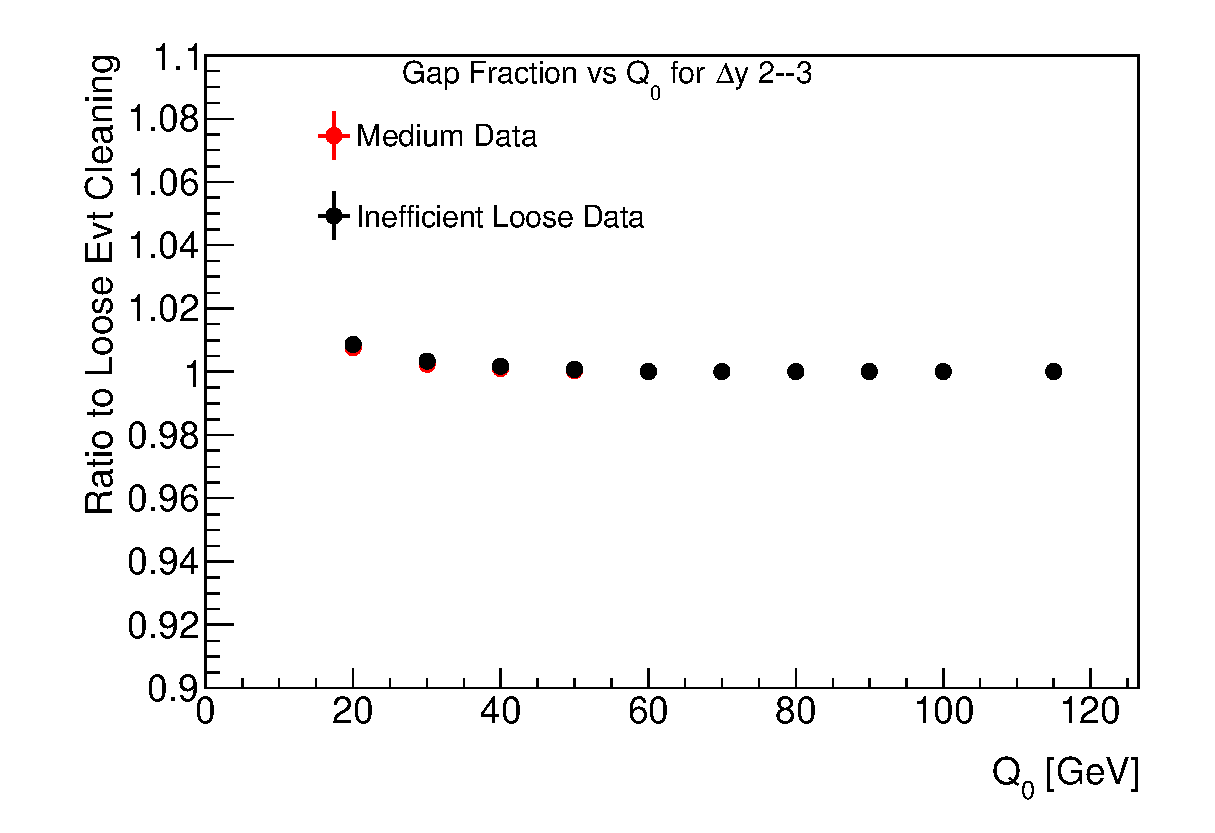
\includegraphics[width=\textwidth]{figures/GBJ2/jetcleaning/Clean_2_3__Q0_Ratio_MediumLoose_Evt_Data.eps}
        \end{subfigure}%
\caption[Comparison loose between and medium cleaning cuts on the gap fraction and average number of jets]{

The ratio of (a) the gap fraction  and (b) the average number of jets in the rapidity region bounded by the dijet as a function of \dy{} for the MC and data with medium jet cleaning cuts compared to loose cleaning cuts at the event-level.
\label{GBJ2:JetCleaning:gap_ML}}
\end{figure}


\begin{figure}
\centering
        \begin{subfigure}[b]{0.5\textwidth}
                \centering
                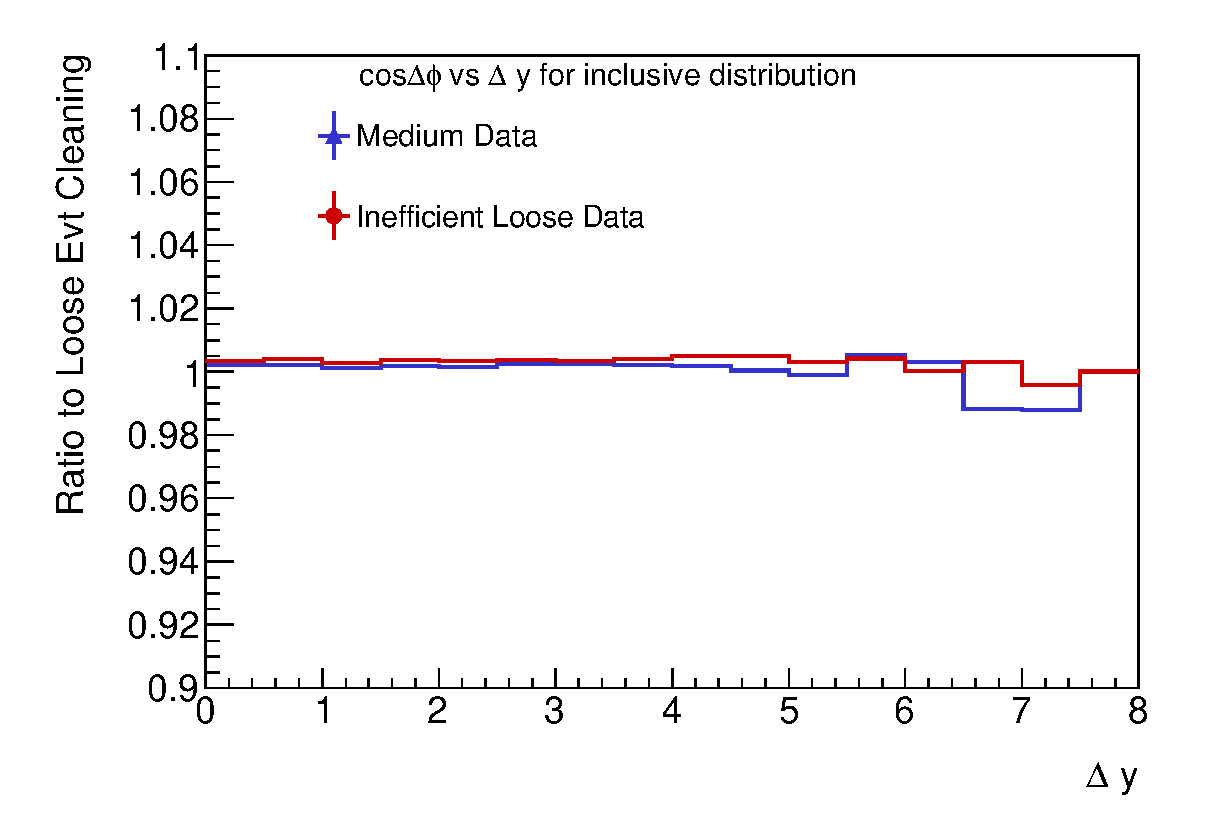
\includegraphics[width=\textwidth]{figures/GBJ2/jetcleaning/Clean___cosdPhi_deltaY_Ratio_MediumLoose_Evt_Data.eps}
        \end{subfigure}%
        \begin{subfigure}[b]{0.5\textwidth}
                \centering
                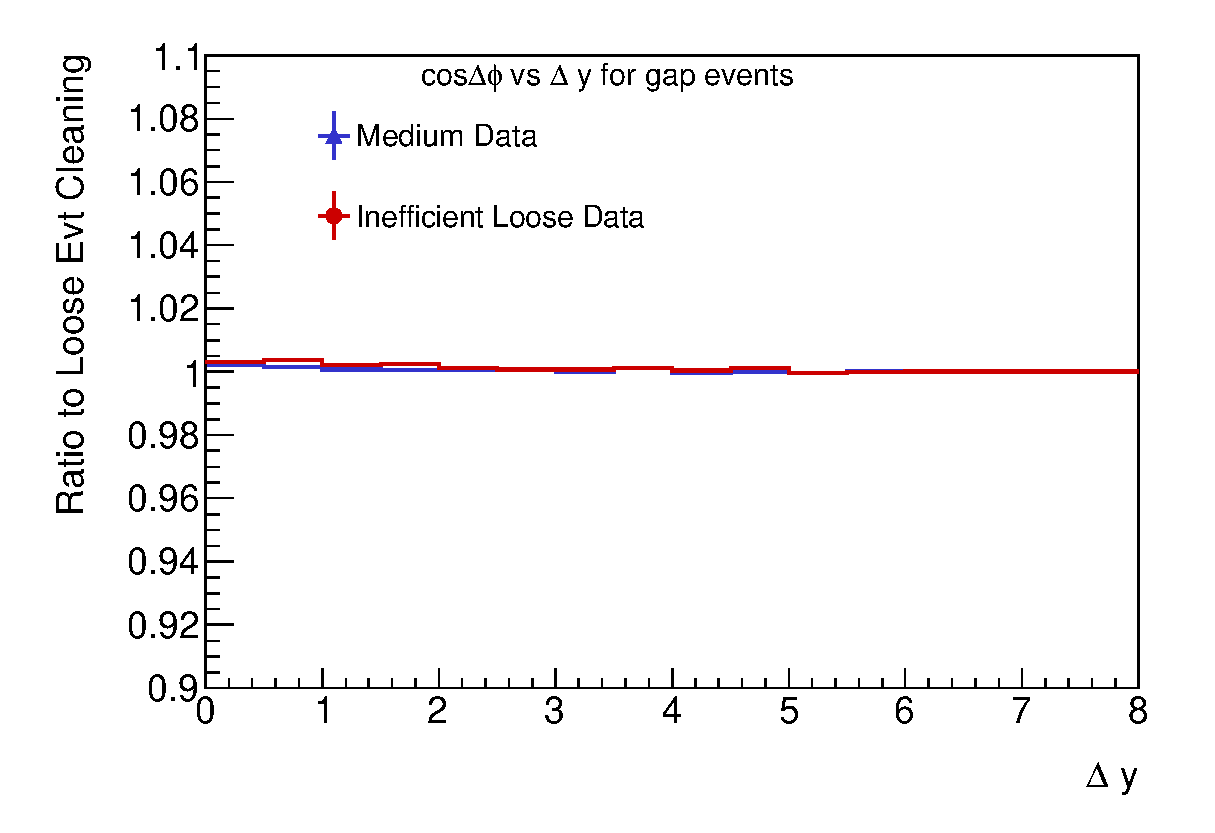
\includegraphics[width=\textwidth]{figures/GBJ2/jetcleaning/Clean___cosdPhi_deltaY_gap_Ratio_MediumLoose_Evt_Data.eps}
        \end{subfigure}%
\caption[Comparison loose between and medium cleaning cuts on \mean{\cosdphi{}}]{
The ratio of \mean{\cosdphi{}} as a function of \dy{} for (a) inclusive and (b) gap events for the MC and data with medium jet cleaning cuts compared to loose cleaning cuts at the event-level.
\label{GBJ2:JetCleaning:cos_ML}}
\end{figure}


\begin{figure}
\centering
        \begin{subfigure}[b]{0.5\textwidth}
                \centering
                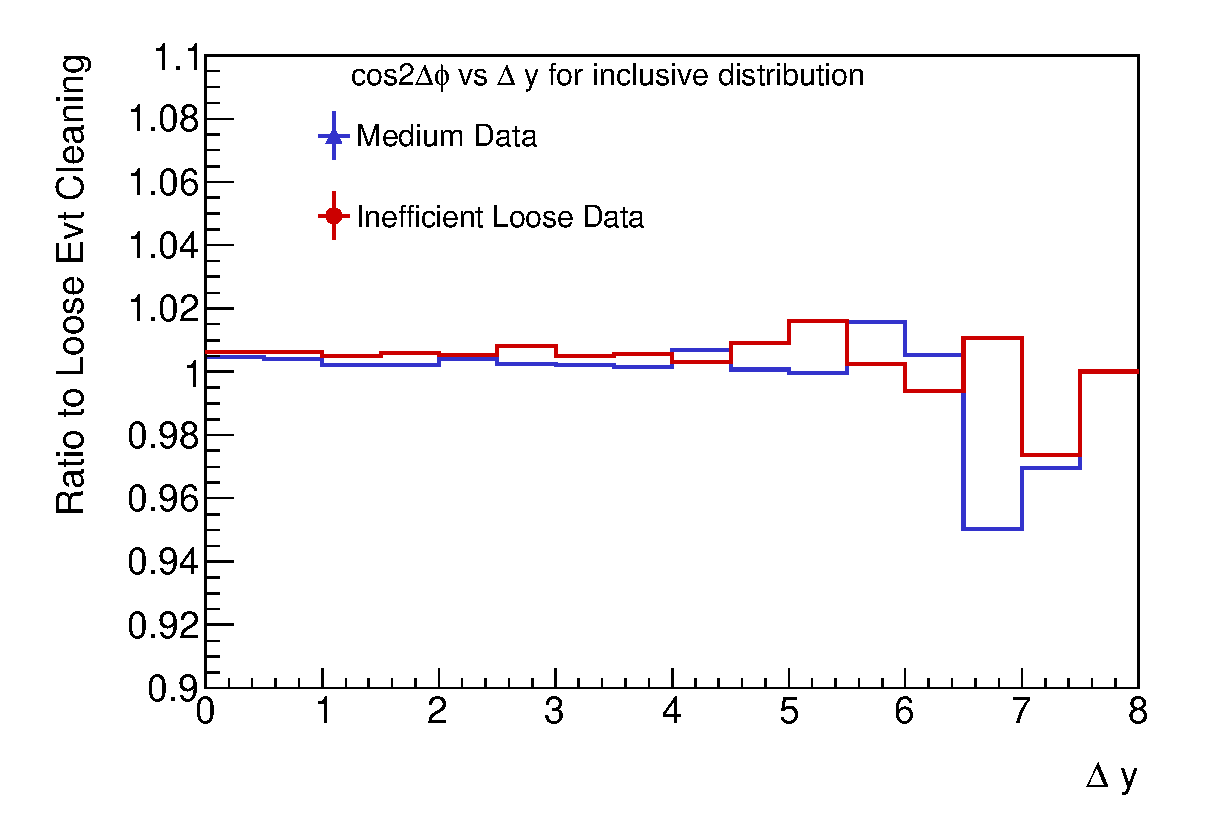
\includegraphics[width=\textwidth]{figures/GBJ2/jetcleaning/Clean___cos2dPhi_deltaY_Ratio_MediumLoose_Evt_Data.eps}
        \end{subfigure}%
        \begin{subfigure}[b]{0.5\textwidth}
                \centering
                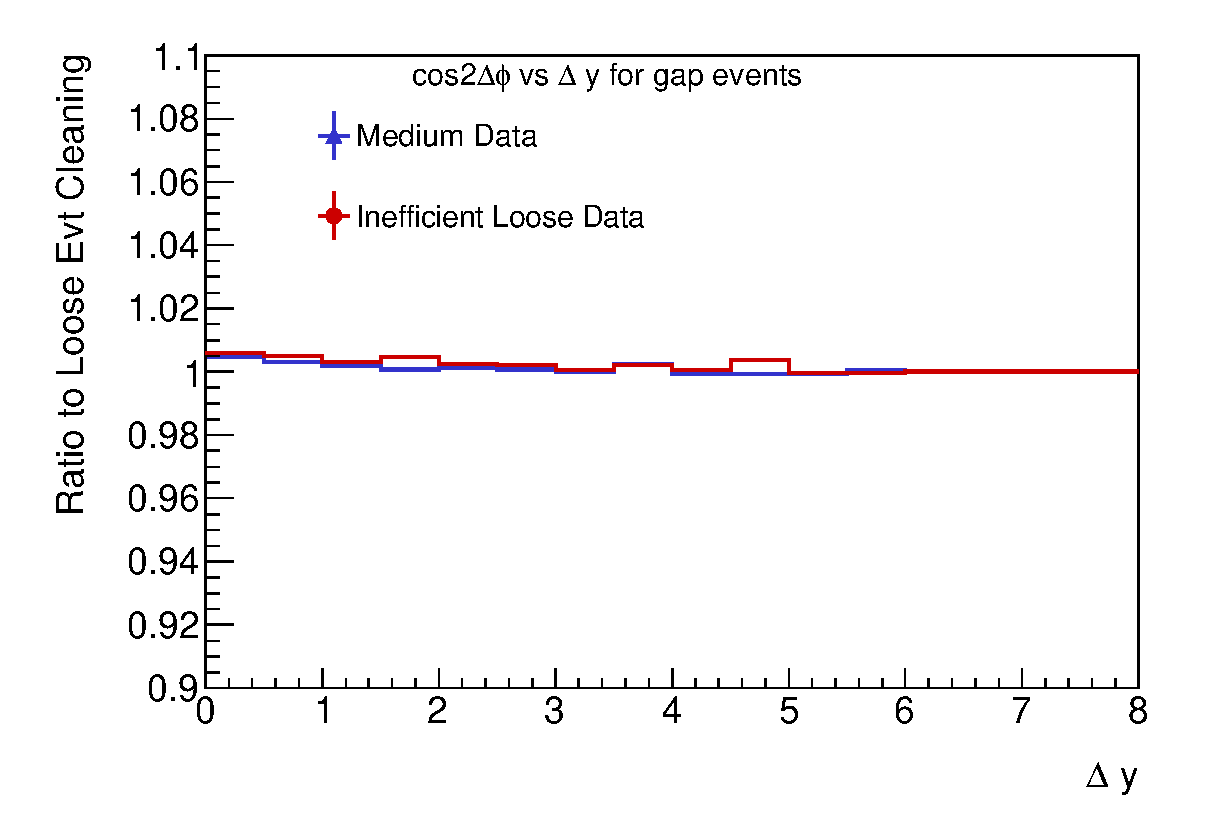
\includegraphics[width=\textwidth]{figures/GBJ2/jetcleaning/Clean___cos2dPhi_deltaY_gap_Ratio_MediumLoose_Evt_Data.eps}
        \end{subfigure}%
\caption[Comparison loose between and medium cleaning cuts on \mean{\costwodphi{}}]{
The ratio of \mean{\costwodphi{}} as a function of \dy{} for (a) inclusive and (b) gap events for the MC and data with medium jet cleaning cuts compared to loose cleaning cuts at the event-level.

\label{GBJ2:JetCleaning:cos2_ML}}
\end{figure}


\begin{figure}
\centering
        \begin{subfigure}[b]{0.5\textwidth}
                \centering
                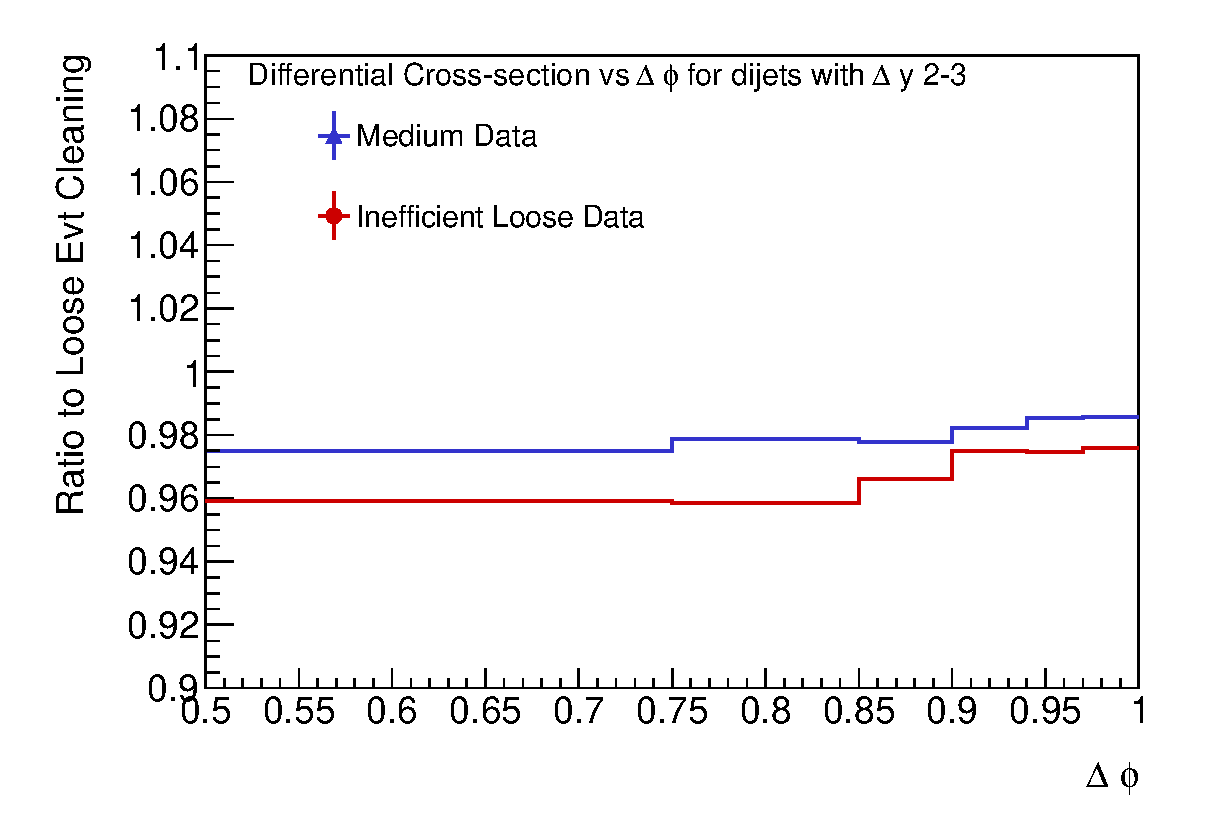
\includegraphics[width=\textwidth]{figures/GBJ2/jetcleaning/Clean___dPhi__2_3_Ratio_MediumLoose_Evt_Data.eps}
        \end{subfigure}%
        \begin{subfigure}[b]{0.5\textwidth}
                \centering
                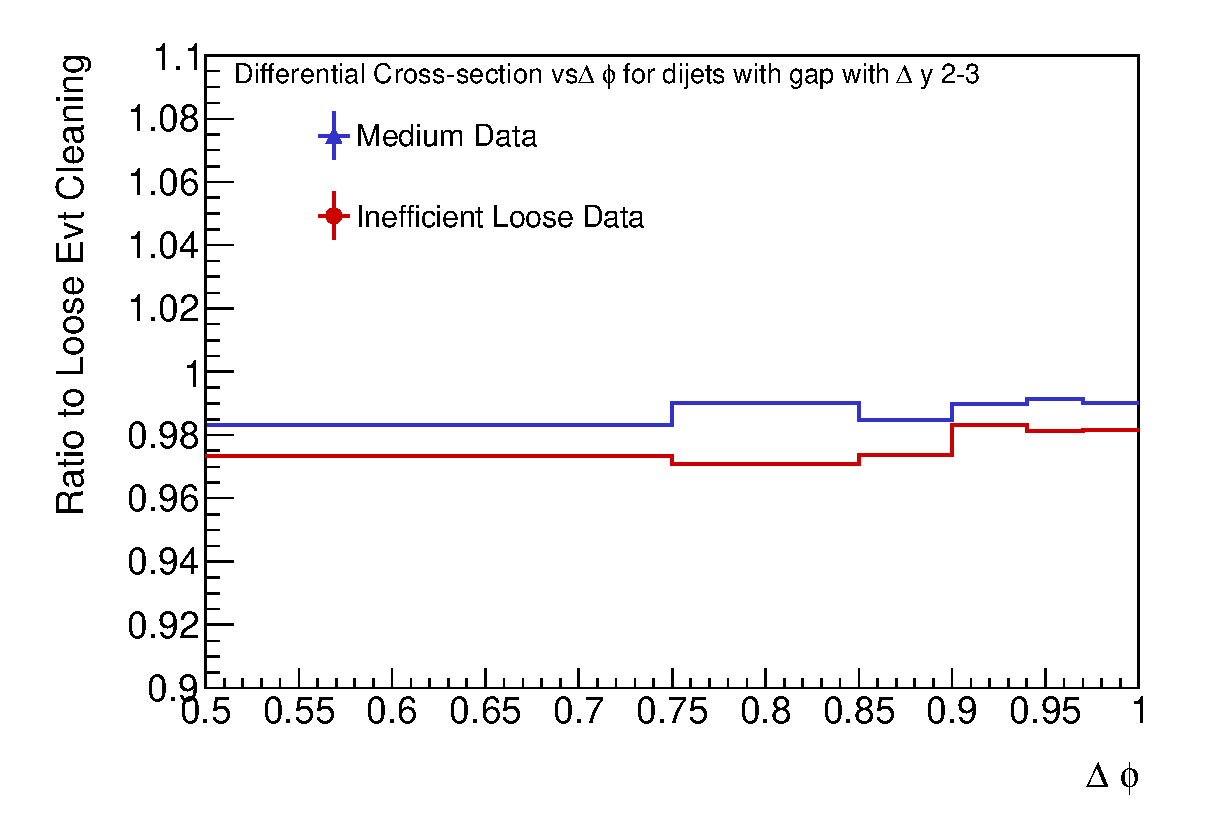
\includegraphics[width=\textwidth]{figures/GBJ2/jetcleaning/Clean___dPhi_gap__2_3_Ratio_MediumLoose_Evt_Data.eps}
        \end{subfigure}%
\caption[Comparison loose between and medium cleaning cuts on \dphiDist{}]{

The ratio of \dphiDist{} for  $2<\dy{}<3$ for (a) inclusive and (b) gap events for the MC and data with medium jet cleaning cuts compared to loose cleaning cuts at the event-level.

\label{GBJ2:JetCleaning:dphi23_ML}}
\end{figure}


%
%\begin{figure}
%\centering
%\mbox{
%              \subfigure[]{\epsfig{figure=figures/GBJ2/jetcleaning/Clean___dPhi__4_5_Ratio_MediumLoose_Evt_Data.eps,width=0.5\textwidth}}\quad
%              \subfigure[]{\epsfig{figure=figures/GBJ2/jetcleaning/Clean___dPhi_gap__4_5_Ratio_MediumLoose_Evt_Data.eps,width=0.5\textwidth}}\quad
%                              }
%\caption[]{
%The ratio of the \dphi{} distribution for \dy{} of 4--5 for (a) inclusive and (b) gap events for the MC and data with medium jet cleaning cuts compared to loose cleaning cuts at the event-level.
%
%\label{GBJ2:JetCleaning:dphi45_ML}}
%\end{figure}
%
%
%
%\begin{figure}
%\centering
%\mbox{
%              \subfigure[]{\epsfig{figure=figures/GBJ2/jetcleaning/Clean___dPhi__7_8_Ratio_MediumLoose_Evt_Data.eps,width=0.5\textwidth}}\quad
%              \subfigure[]{\epsfig{figure=figures/GBJ2/jetcleaning/Clean___dPhi_gap__7_8_Ratio_MediumLoose_Evt_Data.eps,width=0.5\textwidth}}\quad
%                              }
%\caption[]{
%The ratio of the \dphi{} distribution for \dy{} of 4--5 for (a) inclusive and (b) gap events for the MC and data with medium jet cleaning cuts compared to loose cleaning cuts at the event-level.
%
%\label{GBJ2:JetCleaning:dphi78_ML}}
%\end{figure}
%
